\begin{graphicspathcontext}{{./chapters/hmas/imgs/},{./chapters/hmas/imgs/auto/},\old}

\begin{frame}{What is a Complex System?}
	\begin{columns}
		\begin{column}{.5\linewidth}
			\begin{block}{Key characteristics \cite{Simon.96}}
				\begin{description}
				\item[Many heterogeneous components] interacting locally
				\item[Non-linear interactions] small causes, large effects
				\item[Emergent behaviour] global properties not present in individual components
				\item[Feedback loops] components react to the system state
				\item[Natural hierarchy] complexity is organised in levels of abstraction
				\end{description}
			\end{block}
		\end{column}
		\begin{column}{0.44\linewidth}
			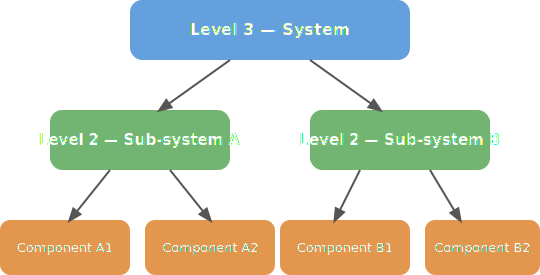
\includegraphics{hmas_complex_system_levels}
		\end{column}
	\end{columns}
\end{frame}

\sidecite{Simon.96}
\begin{frame}{Simon's Near-Decomposability Principle}
	\begin{alertblock}{H.~A.~Simon, 1962}
		``Complexity frequently takes the form of a hierarchy. A hierarchy is a system composed of interrelated sub-systems, each of the latter being in turn hierarchic''
	\end{alertblock}
	\vspace{.25cm}
	\begin{block}{Two types of interactions}
		\begin{description}
		\item[Intra-subsystem] Frequent, strong — define the identity of
		each sub-system
		\item[Inter-subsystem] Rare, weak — couple sub-systems together
		to form a higher level
		\end{description}
	\end{block}
	\vspace{.25cm}
	\begin{exampleblock}{Consequence for modelling}
		A model must be able to represent \Emph{multiple levels of abstraction} simultaneously
	\end{exampleblock}
\end{frame}

\begin{frame}{Why Multiagent Systems for Complex Systems?}
	\smaller
	\begin{columns}
		\begin{column}{.5\linewidth}
			\begin{block}{MAS are well suited because\ldots}
				\begin{itemize}
				\item Agents naturally represent \Emph{heterogeneous} autonomous entities
				\item \Emph{Local interaction rules} naturally produce emergent phenomena
				\item \Emph{Decentralised control} mirrors real complex systems
				\item No single point of failure; \Emph{resilient} by design
				\end{itemize}
			\end{block}
			\begin{alertblock}{But\ldots}
				Classical MAS treat agents as \Emph{atomic} and \Emph{single-level}.
				They cannot represent a component that is simultaneously \emph{an agent}
				and \emph{a system}
			\end{alertblock}
		\end{column}
		\begin{column}{.5\linewidth}
			\begin{block}{Multilevel Need}
			\hspace{.25cm}
			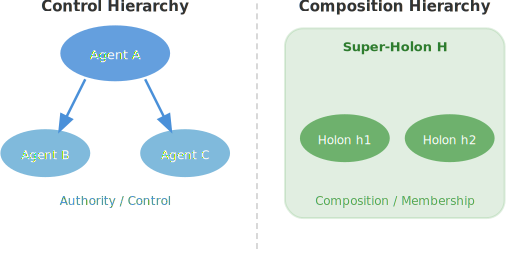
\includegraphics{hmas_two_hierarchies}
			\end{block}
		\end{column}
	\end{columns}
\end{frame}

\begin{frame}{{Two Kinds} of Hierarchy in MAS}
	\begin{center}
		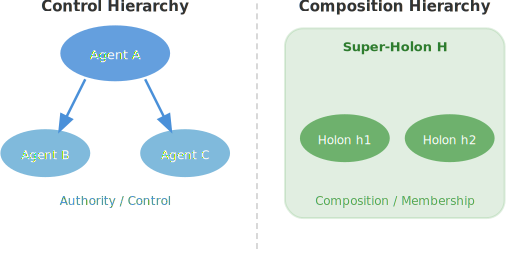
\includegraphics[width=.5\linewidth]{hmas_two_hierarchies}
	\end{center}
	\smaller
	\begin{columns}
		\begin{column}{.5\linewidth}
			\begin{block}{Control Hierarchy}
				\begin{itemize}
				\item A relationship of \Emph{authority} between agents
				\item A manager agent issues orders to subordinate agents
				\item Agents remain \emph{distinct} entities
				\end{itemize}
			\end{block}
		\end{column}
		\begin{column}{.5\linewidth}
			\begin{block}{Composition Hierarchy}
				\begin{itemize}
				\item Agents are \Emph{physically composed} of other agents
				\item A super-agent \emph{contains} member agents
				\item The same entity is viewed at different granularities
				\end{itemize}
			\end{block}
		\end{column}
	\end{columns}
\end{frame}

\end{graphicspathcontext}

\endinput

